\documentclass[a4paper,twocolumn,11pt,unpublished]{quantumarticle}
\pdfoutput=1

\usepackage{mathtools}
\usepackage{amsmath}
\usepackage{amssymb}
\usepackage{amsthm}
\usepackage[normalem]{ulem}
\usepackage{comment}
\usepackage{env}
\usepackage{enumitem}


\newtheorem{protocol}{Protocol}
\newcommand{\Accept}{\mathsf{Accept}}
\newcommand{\Reject}{\mathsf{Reject}}
\newcommand{\Pauli}{\mathcal P}
\newcommand{\Hilbert}{\mathcal H}
\newcommand{\Clifford}{\mathcal C}
\newcommand{\sgn}{\mathrm{sgn}}
\newcommand{\np}{m}
\newcommand{\CEPS}{$\mathcal C$PS}
\newcommand{\mCEPS}{\mathcal{C}\text{PS}}
\newcommand{\STAB}{STAB}
\newcommand{\GS}{GS}
\newcommand{\HGS}{HGS}
\newcommand{\pdist}{\mathcal D} % notation for distribution of Pauli measurements for DFE of qubit i (subject to change)
\newcommand{\qdist}{\mu} % notation for qubit choice for DFE (subject to change)
\newcommand{\jdist}{\mathcal D} % joint distribution (subject to change)
\newcommand{\dist}{\mathcal G} % joint distribution (subject to change)
\newcommand{\copyindex}{j}
\newcommand{\qubit}{i}
\renewcommand{\O}{\mathcal O}
\newcommand{\ketbra}[1]{\ket{#1}\!\bra{#1}}
\newcommand{\abs}[1]{\left|#1\right|}
\title{Efficient certification of intractable quantum states with few Pauli measurements}
% \title{Verification of universal quantum computations through single-qubit tomography}

\author{Sami Abdul-Sater}
\author{Maxime Garnier}
\author{Thierry Martinez}
\author{Harold Ollivier}
\author{Ulysse Chabaud}
\affiliation{INRIA, DIENS, Ecole Normale Supérieure, PSL University, CNRS, 45 rue d’Ulm, Paris 75005, France}

\begin{document}


\begin{abstract}
    Verification of quantum computations is crucial as experiments advance toward fault-tolerant quantum computing. Yet, no efficient protocol exists for certifying states generated in the Magic-State Injection model — the foundation of several fault-tolerant quantum computing architectures.
    Here, we introduce an efficient protocol for certifying \textit{Clifford-enhanced Product States}, a large class of quantum states obtained by applying an arbitrary Clifford circuit to a product of single-qubit, possibly magic, states.
    Our protocol only requires single-qubit Pauli measurements together with efficient classical post-processing, and has efficient sample complexity in both the independent (i.i.d.) and adversarial (non-i.i.d.) settings.
    % It is conducted by 
This fills a key gap between Pauli-based certification schemes for stabilizer or (hyper)graph states and general protocols demanding non-Pauli measurements or classically intractable information about the target state. 
    Our work provides the first efficient, Pauli-only certification protocol for the Magic-State Injection model, leading to practical verification of universal quantum computations under minimal experimental assumptions.
\end{abstract}


\maketitle


\section{Introduction}


Quantum computers' promises and potential to outperform classical ones for certain computational tasks \cite{S94algorithms, G96fast, F82simulating, F86quantum, D85quantum, HCMP25vast} has generated rapid progress in the field \cite{P18quantum, EP25mind}.
Increasingly complex devices and experiments are being realized across various platforms \cite{NLDC22beating, AAAA25constructive, DBMA25breaking}. 
However, these developments must be accompanied by the design of reliable techniques to \emph{certify the outputs of quantum experiments} and \emph{verify the correctness of quantum computations} \cite{EHWR20quantum, BPY25quantum, PYBB24benchmarking}, especially in the context of delegated quantum computing, in which quantum computing is envisioned as a cloud service provided by a potentially untrusted party \cite{GKK19verification}.

Verification of quantum computations and certification of quantum states are closely related tasks, particularly for models of computation that proceed by \emph{preparing a specific resource state} and then performing a sequence of adaptive measurements on it to drive the computation. 
Prominent examples include \emph{Measurement-Based Quantum Computation} (MBQC) \cite{RB01one, DKP07measurement, BBDR09measurement} and, even more so, \emph{Magic-State Injection} (MSI) \cite{BK04universal}. 
In the latter, a target resource state is obtained by applying a Clifford circuit to a product of single-qubit states---some of which may be non-stabilizer, or ``magic'', states---followed by adaptive Pauli measurements that realize universal computation. 
Magic-State Injection has become a leading paradigm for \emph{fault-tolerant quantum computation} \cite{DBMA25breaking, G23cleaner, AAAA22suppressing}, as it cleanly separates the easily error-correctable Clifford operations from the costly non-Clifford resources that enable universality.

While verification and certification have been extensively studied in the context of MBQC \cite{TM17verification, TMMM18resource, ZH19efficient, ZH18efficient, LZH23robust}, no efficient protocol is available for the verification of computations based on Magic-State Injection. 
This gap is particularly notable given that MSI underlies several practical architectures for scalable, fault-tolerant quantum computing (FTQC) \cite{MGCM25ibm, GSJ24magic}.

In this paper, we address this gap and introduce a sample-efficient and time-efficient protocol using non-adaptive, single-qubit Pauli measurements for certifying arbitrary quantum states of the form
\begin{equation}
    \label{eq:intro:CliffordProductStates}
    \ket{\Psi} = C\!\left(\bigotimes_{i=1}^n \ket{\psi_i}\right),
\end{equation}
where $C$ is an $n$-qubit Clifford circuit and $\ket{\psi_i}$ are arbitrary single-qubit states, potentially magic states. 
We refer to this family as \emph{Clifford-enhanced Product States} (\CEPS, inspired by \cite{LHD24quantum}), as it naturally arises by considering an arbitrary $n-$qubit product state and applying an arbitrary Clifford circuit on it, encompassing resource states for Magic-State Injection.
This class generalizes several standard classes of states: restricting each $\ket{\psi_i}$ to stabilizer states yields the family of \emph{stabilizer states}; further restricting $C$ to products of controlled-$Z$ gates yields \emph{graph states}, a subset of stabilizer states and a special case of \emph{hypergraph states} when the hypergraph is a simple graph.
These relations are illustrated in Fig.~\ref{fig:diagram}.
\begin{figure}[t]
    \centering
    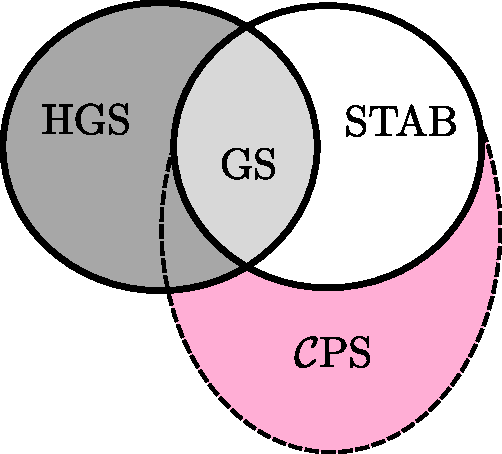
\includegraphics[width=0.7\linewidth]{figures/diagrams.pdf}
    \caption{Relationship between Clifford-enhanced Product States (\CEPS), Stabilizer States (\STAB), Graph States (\GS), and Hypergraph States (\HGS). \CEPS~reduces to \STAB~if the product state contains only stabilizer states ; and it furthermore reduces to \GS~if in addition the Clifford circuit is only made of $CZ$.
    A \HGS~is a \GS~if the underlying hypergraph is a graph.
    % \STAB~(including \GS) with Pauli measurements are not enough together to yield universal quantum computation. \HGS$\backslash$\STAB~and \CEPS$\backslash$\STAB~do have this property, but \CEPS~is more compatible with most FTQC architectures.
    }
    \label{fig:diagram}
\end{figure}

Our protocol allows us to efficiently certify any $n$-qubit Clifford-enhanced Product State using only Pauli measurements, both in the i.i.d.\ case
--- where the state preparations are independent and identical across samples ---
and the general case ---  where samples may be correlated, with a number of samples that scales polynomially in $n$.


\paragraph{Related works.}
State certification protocols typically involve a \emph{prover--verifier} setting, where a verifier with limited computational capabilities (often restricted to single-qubit quantum measurements and classical processing) estimates the fidelity of a quantum state with a target state within a precision $\epsilon$ and failure probability~$\delta$, based on $N$ copies.
In this work, we focus on the practically relevant setting where the verifier is restricted to single-qubit Pauli measurements, as these are natively available in most qubit-based architectures.
The main performance metric of a state certification protocol is its sample complexity, i.e.\ the scaling of $N$ with respect to system size~$n$, precision~$\epsilon$, and failure probability~$\delta$. On top of sample complexity, an efficient certification protocol also needs to be time-efficient, i.e.\ that the running time of its classical post-processing scales at most polynomially with the size of the target state.

Quantum state certification is well studied for resource states of MBQC, and its generalization to Hypergraph-Based MBQC.
In these computational models, the resource state is a (hyper)graph state, prepared by entangling $\ket{+}$ states according to a (hyper)graph structure using (multi-)controlled-$Z$ gates.
Both classes of states can be certified efficiently using only Pauli measurements on $N \in \mathcal{O}(\log(1/\delta)/\epsilon)$ samples \cite{ZH18efficient}.
However, both models present caveats in practice. Firstly, even though graph states can be verified efficiently with Pauli measurements, MBQC would ultimately require non-Pauli measurements to achieve universal QC (only Clifford computations is possible if restrained to Pauli measurements \cite{DKP07measurement}).  Secondly, even though hypergraph-based MBQC with Pauli measurements achieves universality \cite{TMH18quantum}, the preparation of hypergraph states involves multi-qubit controlled-$Z$ gates (non-Clifford), challenging to implement within standard fault-tolerant architectures.

These protocols remain particularly attractive due to their efficiency, which can be explained by their exploitation of the (quasi-)stabilizer structure of the underlying states \cite{ZH19efficient}, ensuring that certain sets of Pauli measurements yield deterministic outcomes on the target state.
This property indeed allows the verifier to construct simple pass/fail tests that directly witness fidelity, with an optimal scaling in $n, \epsilon, \delta$ \cite{ZH19efficient}, even in the presence of noise \cite{LZH23robust}.

However, such stabilizer-based reasoning does not extend to the MSI model.
Intuitively, when the target state involves magic (non-stabilizer) components, there is no trivial way of producing such deterministic correlations using sets of Pauli measurements.
% no large enough set of Pauli measurements can produce such deterministic correlations.
%As a result, to the best of our knowledge, no known efficient Pauli-only certification protocol exists for the MSI model.

On the other hand, more general protocols that aim to certify \textit{any} quantum state have also been studied.
Traditional techniques such as tomography or Direct Fidelity Estimation scale exponentially with the system size \cite{FL11direct, FOS24optimal, SLP11practical}. Instead general-purpose certification protocols based on fidelity witnessing using Pauli measurements are available for ``almost all'' states~\cite{HPS24certifying} (and even all states when using adaptive measurements~\cite{GHO25few}) but they assume query access to the target state amplitudes in the computational basis. However, computing the amplitudes of the output state of a quantum circuit is $\#P-$hard in the worst case \cite{A04quantuma, BFNV18quantum}, and in particular for target states relevant for MSI \cite{YJS18quantum}. This implies that, while potentially being sample-efficient, the protocols \cite{HPS24certifying,GHO25few} would not be time-efficient for all resource states of MSI (unless $P=P^{\#P}$).

 

% [Add impact]
As such, our protocol bridges an important gap, providing an efficient way to certify quantum states in a setting compatible with MSI, where target state amplitudes are classically intractable. It thus offers a practical tool for experimental implementations where Pauli measurements are the natural measurement primitive.\\

The rest of the paper is structured as follows. We provide preliminary background in section \ref{sec:prelim}: clarification on the assumptions made on the prover are given in \ref{subsection:prelims:iid}, while \ref{subection:prelims:physical setting} discusses the physical setting --- Pauli measurements, quantum computation \emph{via} MSI --- and \ref{subsection:prelims:math} presents the mathematical tools involved in the development of the protocol. The protocol itself
for efficiently certifying Clifford-enhanced Product States
is introduced in section \ref{section:certification}. It is then shown in section \ref{section:verification} that the guarantees of the state certification protocol still hold in the adversarial setting modulo an increase of the number of samples. Section \ref{section:VQC} explains how to use this protocol as a subroutine to perform efficient verification of universal quantum computations using Pauli measurements in the MSI model. We conclude in section \ref{section:conclusion}.

\section{Preliminaries}
\label{sec:prelim}
In this work, we consider systems composed of qubits whose state is a normalized vector in a two-dimensional Hilbert space $\Hilbert = \mathbb C ^2$, with composite systems described by tensor products of such spaces. For a more general introduction to quantum information science, we refer the reader to \cite{NC00quantum}.
% Note that all the results of this paper can without loss of generality be applied to any finite-dimensional Hilbert space (\emph{i.e}, the generalization of the protocols and results from qubits to \emph{qudits} is straightforward by adapting the notations).

% What we mean by certification/verification
% \begin{itemize}
%     \item State certification = iid prover and check that prepared state is close to target with good probability 
%     \item State verification: figure of merit from hypothesis testing 
% \end{itemize}

% Our setting:
% \begin{itemize}
%     \item Receive and measure
%     \item Universal model of quantum computation: magic-state injection
%     \item Pauli measurements, Clifford unitaries: \ref{subsection:prelims:Pauli meas}.
% \end{itemize}

% Our tools:
% \begin{itemize}
%     \item Fidelity and trace distance: done in \ref{subsection:prelims:Fidelity}.
%     \item Concentration bounds \ref{subsection:prelim:concentration}
%     \item Optimal single-qubit fidelity estimation: done in \ref{subsection:prelims:DFE}.
%     \item Fidelity witnesses for product states: done in \ref{subsection:prelims:witness}.
%     \item Backpropagation: done in \ref{subsection:prelims:backprop}.
% %    \item $k$-colorability
%     \item Sampling without replacement in robust hypothesis testing
% \end{itemize}

\subsection{State Certification and Verification}
\label{subsection:prelims:iid}
In this work, we distinguish between the notions of \emph{state certification} and \emph{state verification}.
Both tasks aim to determine whether a state preparation is \emph{faithful} to a given target state, that is, whether the prepared states are sufficiently close to the target according to suitable figures of merit introduced hereafter.
The difference lies in the assumptions made about the source producing these states.

In \emph{state certification}, we assume that the prover (or source) prepares the states in an \emph{independent and identically distributed} (\emph{i.i.d.}) manner, and the task is to check that such preparations are close to the target state with high probability \cite{FL11direct, FOS24optimal, CGKM21efficient, GHO25few, HPS24certifying}.
In contrast, we use \emph{state verification} to refer to the more general situation in which no i.i.d.\ assumption is made, the prover could be adversarial, and the prepared systems may exhibit correlations. In Lemma \ref{lemma:prelim:iid} we recall a result from \cite{FKMO24learning} which allows to lift any learning task in the \emph{i.i.d} scenario to the \emph{non-i.i.d} one, which allows us to employ a similar protocol for state \emph{certification} and state \emph{verification}. Note that the adversarial scenario is sometimes dealt with in an hypothesis testing framework instead \cite{ZH18efficient, ZH19efficient, LZH23robust, LZ25universal}.
% In this case, the goal is typically reformulated within a \emph{hypothesis-testing} framework (honest vs. dishonest prover/source), where one assesses the preparation procedure through a figure of merit quantifying the confidence with which the target hypothesis can be accepted \cite{ZH18efficient, ZH19efficient, LZH23robust, LZ25universal}.
% This broader setting is often called the \emph{adversarial scenario}, as it encompasses both naturally correlated and potentially malicious sources.

\subsection{Physical setting of the work}
\label{subection:prelims:physical setting}

\subsubsection{Receive-and-measure}
\label{subection:prelims:RnM}

In the considered setting, the protocol follows a \emph{receive-and-measure} structure. The verifier is a weakly quantum entity: it can receive qubits, perform Pauli measurements, and carry out (randomized) classical post-processing of the outcomes. The prover, in contrast, is assumed to prepare and send quantum systems to the verifier; the only structural assumption that may be imposed is the \emph{i.i.d.}\ one, where each transmitted subsystem is identically and independently prepared (see the paragraph above).
At each round, the verifier receives a quantum register from the prover, applies a measurement corresponding to a chosen Pauli observable, and records the outcome. From the resulting statistics, the verifier computes empirical expectation values and derives a numerical quantity used to certify that the remaining (unmeasured) subsystem is close, in a suitable metric, to the desired target state with high probability.

\subsubsection{Pauli measurements}
\label{subsection:prelims:Pauli meas}

The single-qubit Pauli operators form the set ${I, X, Y, Z}$, and the $n$-qubit Pauli group $\Pauli_n$ is defined as all $n-$tensor products of these operators up to global phases ${\pm 1, \pm i}$. The Clifford group $\Clifford_n$ is the normalizer of $\Pauli_n$ in the unitary group, i.e., the set of unitaries that map Pauli operators to Pauli operators under conjugation. Namely, for any $P\in\Pauli_n$ and $C\in\Clifford_n$, we have $CPC^\dagger\in \Pauli_n$.
A Pauli measurement corresponds to measuring an observable $P \in \Pauli_n$ with eigenvalues $\pm 1$. Since any multi-qubit Pauli operator is a tensor product of single-qubit Paulis, such a measurement can be implemented by measuring each qubit in the appropriate single-qubit Pauli basis and taking the product of the individual outcomes. This procedure reproduces exactly the same measurement statistics and post-measurement states as a direct joint measurement of $P$.

\subsubsection{Universal QC via Magic-State Injection}
\label{subection:prelims:MSI}

In this work, we use the fact that universal quantum computation can be performed with Clifford unitaries and adaptive Pauli measurements, starting with stabilizer states and non-stabilizer $T\ket + = 1/\sqrt2(\ket0+e^{i\pi/4}\ket1)$ states. Those are often called \emph{magic states}, where $T$ is the $\pi/4-$rotation around the $Z$ axis of the Bloch Sphere, $T=R_z(\pi/4)$. This is the "Magic-State Injection" (MSI) model, proved to be universal for quantum computation \cite{BK04universal}. As stated in the introduction, it has become a particularly relevant model in the development of fault-tolerant architectures. To perform a computation in this model, a state of the form $C\left(\bigotimes_{i=1}^n \ket{\psi_i}\right)$ must thus be prepared, where the single-qubit states $\ket{\psi_i}$ can be stabilizer or magic states, and adaptive Pauli measurements must be performed. This is depicted on figure \ref{fig:MSI}. The quantum state before measurements has thus the structure of the $\mCEPS$ class, which is why certifying states of this class is crucial to verify MSI-based quantum computations, which is the whole subject of this work.
% The class of resource states that this model generates is indeed
% In this model, the resource state that undergoes adaptive Pauli measurements to yield the outcome of the computation is indeed of the form $C\left(\bigotimes_{i=1}^n \ket{\psi_i}\right)$ for single-qubit states $\ket{\psi_i}$ that can be stabilizer or magic states.
% This is precisely what is captured by our definition of the Clifford-enhanced Product States.
 
\begin{figure}
    \centering
    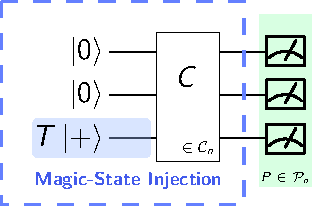
\includegraphics[width=\linewidth]{figures/MSI.pdf}
    \caption{Magic-State Injection model. The blue dashed box captures the fact that teh state prior to measurements has the structure of the $\mCEPS$ class introduced previously. The green box consists of a layer of adaptive single-qubit Pauli measurements to drive the computation.}
    \label{fig:MSI}
\end{figure}
\subsection{Mathematical tools}
\label{subsection:prelims:math}
\subsubsection{Fidelity and trace distance}
\label{subsection:prelims:Fidelity}

To quantify the closeness between two quantum states $\rho$ and $\sigma$, two fundamental quantities are widely used: \emph{fidelity} and \emph{trace distance}.

The fidelity is defined as
\[
F(\rho, \sigma) = \left( \Tr \sqrt{\sqrt{\rho}\,\sigma\,\sqrt{\rho}} \right)^2 .
\]
It measures the overlap between $\rho$ and $\sigma$, and satisfies $0 \leq F(\rho, \sigma) \leq 1$, with equality $F(\rho, \sigma) = 1$ if and only if $\rho = \sigma$. When one of the two states is pure, say $\sigma = \ketbra{\psi}$, then we write with an abuse of notation $F(\rho, \ket\psi)$ and it simplifies to
\begin{equation}
\label{fidover}
F(\rho, \ket{\psi}) = \Tr[\rho\ketbra\psi]= \bra{\psi}\rho\ket{\psi}.
\end{equation}

The trace distance is defined as 
\begin{equation}    
D(\rho, \sigma) = \frac{1}{2}\|\rho - \sigma\|_1 = \frac{1}{2}\Tr|\rho - \sigma|,
\end{equation}
and constitutes a metric on the space of operators. It also admits a direct operational interpretation: it characterizes the largest possible difference in outcome probabilities that any measurement can produce between the two states,
\begin{equation}
D(\rho, \sigma) = \max_{0 \le E \le \mathbb I}
\abs{\Tr[E(\rho - \sigma)]}
\end{equation}
Here the maximization is taken over all measurement effects $E$ such that $0 \le E \le \mathbb I$, corresponding to the "yes" outcome of a two-outcome POVM $\{E, \mathbb I - E\}$. Hence, the trace distance quantifies the maximal statistical distinguishability between $\rho$ and $\sigma$: it is the greatest bias achievable when attempting to tell the two states apart using any physically allowed measurement.


The two quantities are closely related through the \emph{Fuchs--van de Graaf inequalities} \cite{FG97cryptographic}:
\begin{equation}
\label{eq:prelim:fuchsvandegraaf}
1 - \sqrt{F(\rho, \sigma)} \leq D(\rho, \sigma) \leq \sqrt{1 - F(\rho, \sigma)}.
\end{equation}
These inequalities provide a quantitative bridge between the geometric notion of overlap and the operational notion of distinguishability. In particular, if the fidelity between $\rho$ and $\sigma$ is close to one, then the trace distance is necessarily small, ensuring that the two states are practically indistinguishable. 

\subsubsection{Concentration bounds}
\label{subsection:prelim:concentration}
A central task in quantum characterization and verification is the estimation of the fidelity between a prepared quantum state $\rho$ and a known pure target state $\ket{\Psi}$. Though the fidelity is rigorously defined mathematically, in practice one wishes to estimate empirically it by measuring observables and analyze the outcomes. Among the crucial tools to evaluate the accuracy of these methods, we find concentration bounds for empirical averages such as Hoeffding's inequality, presented in Lemma \ref{lemma:prelim:hoeffding}.
\begin{lemma}[Hoeffding's inequality]
\label{lemma:prelim:hoeffding}
    Let $\epsilon>0, N>0$, and
    $x_1, \ldots, x_N$ be i.i.d random variables sampled from a probability distribution $\dist$. On this distribution, let $g:\mathbb R \rightarrow \mathbb R$ be a bounded function, and define $G = \max_{x\in\dist}g(x)-\min_{x\in\dist}g(x)$. Then, the probability that the empirical average $\bar X = \frac 1 N \sum_{i=1}^N g(x_{i})$ and the expected value $X=\mathbb E_{x\sim\dist}[g(x)]$ differ from more than  $\epsilon$ decreases exponentially as 
    \begin{equation}
        \Pr\left[
        \abs{
        \bar X
        -
        X
        }
        \geq \epsilon
        \right]
        \leq 
        \exp{
        \left(
        -2\dfrac{N\epsilon^2}{G^2}
        \right)
        }\; .
    \end{equation}
\end{lemma}

\subsubsection{Direct Fidelity Estimation (DFE)}
\label{subsection:prelims:DFE}


\emph{Direct Fidelity Estimation} (DFE) is a method to estimate the fidelity of a state with respect to a target state using single-copy Pauli measurements sampled according to a probability distribution that is computable from the classical description of the target state \cite{FL11direct}. We here remind the optimal method to do so, following \cite{FOS24optimal}.

Let $\Pauli_n$ denote the group of $n$-qubit Pauli operators, and define the \emph{characteristic function} of a pure state $\ket{\psi}$ as
\begin{equation}
    \chi_\psi: \Pauli_n \to [-1,1], \quad 
    \chi_\psi(P) =
    \frac 1 d
    \Tr[\ketbra{\psi} P]
    .
\end{equation}
We have the expansion
\begin{equation}
\label{expansion}
    \ketbra{\psi}= \sum_{P\in\Pauli_n}
    \chi_\psi(P)\,P.
\end{equation}
The $\ell_1$-norm of the characteristic function is defined by
\begin{equation}
    \norm{\chi_\psi}_1 =\sum_{P\in\Pauli_n} \abs{\chi_\psi(P)} \leq {\sqrt{d}},
\end{equation}
where $d = 2^n$ is the Hilbert space dimension. In particular: stabilizer states satisfy $\norm{\chi_\psi}_1=1$,
    and magic states such as $\ket\psi=T\ket+ = 1/\sqrt 2(\ket0+e^{i\pi/4}\ket 1)$ satisfy $\norm{\chi_\psi}_1=(1+\sqrt2)/2$.
% stabilizer states satisfy $\norm{\chi_\psi}_1 = 1$.

Based on this, we define a probability distribution over Pauli operators as
\begin{equation}
\label{DpsiP}
    \mathcal{D}_\psi(P) = \frac{|\chi_\psi(P)|}{\norm{\chi_\psi}_1}.
\end{equation}
Using these definitions, the fidelity between $\rho$ and $\ket{\psi}$ can be expressed in terms of the characteristic function, using the fact that the fidelity can be written as an overlap when one of the states is pure (see Eq.~\eqref{fidover}), and using the expansion of $\ket\psi$ in the Pauli basis (Eq.~\eqref{expansion}):
\begin{align}    
    F(\rho, \ket{\psi}) 
        &= \Tr[\rho \ketbra{\psi}] 
         = \sum_{P \in \Pauli_n} \chi_\psi(P)\, \Tr[\rho P] \nonumber \\
        &= \sum_{P \in \Pauli_n} |\chi_\psi(P)|\, \sgn(\chi_\psi(P))\, \Tr[\rho P] \nonumber \\
        &= \mathbb{E}_{P \sim \mathcal{D}_\psi}
           \left[
             \norm{\chi_\psi}_1 \, \sgn(\chi_\psi(P)) \, \Tr[\rho P]
           \right].
\end{align}
%
Hence, the estimation of the fidelity $F(\rho, \ket{\psi})$ reduces to estimating the expectation value of a random Pauli observable drawn from $\mathcal{D}_\Psi$. Define
\begin{equation}
    f(P) = \norm{\chi_\psi}_1 \, \sgn(\chi_\psi(P)) \, \Tr[\rho P],
\end{equation}
so that $F(\rho, \ket{\psi}) = \mathbb{E}_{P \sim \mathcal{D}_\psi}[f(P)]$.

By performing repeated Pauli measurements according to $\mathcal{D}_\psi$ and averaging the outcomes, one obtains an unbiased estimator of the fidelity. To achieve additive precision $\epsilon$ and failure probability $\delta$, $N> N' \in O(d\, \epsilon^{-2} \log(1/\delta))$ copies of $\rho$ are sufficient, following Hoeffding's inequality (Lemma \ref{lemma:prelim:hoeffding}). 
The distribution $\mathcal{D}_\psi$ can be sampled from in $O(d)$ time.
For a stabilizer state, $\norm{\chi_\psi}_1=1$ and $\mathcal{D}_\psi$ is the uniform distribution over the $d$ Pauli operators of its stabilizer group (up to signs), which can be sampled from efficiently. In that case, $O(\epsilon^{-2} \log(1/\delta))$ copies of $\rho$ are sufficient, independently of $d$ \cite{DHZ20Optimal}.

Although DFE achieves the information-theoretically optimal scaling for direct fidelity estimation, the measurement cost grows exponentially with the system size $n$ for general target states, since $d = 2^n$. Consequently, this method remains practical only for small-scale quantum systems.

\subsubsection{Fidelity witnesses}
\label{subsection:prelims:witness}
The exponential scaling of direct fidelity estimation with system size motivates the use of alternative approaches for efficient state certification. One such approach relies on the introduction of \emph{robust fidelity witnesses} \cite{CGKM21efficient,UC24efficient,HPS24certifying,GHO25few}, quantities that are easier to estimate while still providing a guaranteed bound on the fidelity.

In particular, a robust fidelity witness $W(\rho, \ket{\psi})$ may satisfy
\begin{equation}
\label{eq: robust fidelity witness}
    f(F(\rho, \ket{\psi}))
    \leq W(\rho, \ket{\psi}) 
    \leq F(\rho, \ket{\psi}) ,
\end{equation}
where $f$ is a continuous function such that $f(1) = 1$. 
The right-hand inequality shows that the witness is a \emph{lower bound} on the true fidelity $F(\rho, \ket{\psi})$, while the left-hand inequality characterizes the region where the witness provides meaningful information, namely where $W(\rho, \ket{\psi}) \ge 0$.

For a target $n$-qubit product state $\ket{\psi}=\bigotimes_{i=1}^n\ket{\psi_i}$, a fidelity witness was introduced in \cite{CGKM21efficient} as
\begin{equation}
    \label{eq:prelims:witness}
    W(\rho, \ket{\psi}) 
    \coloneqq 1 - 
    \sum_{i=1}^{n}
    \big(1 - F(\rho_i, \ket{\psi_i})\big),
\end{equation}
where $\rho_i$ denotes the single-qubit reduced state of $\rho$ obtained by tracing out all other subsystems but the $i-$th one.
This expression combines local fidelities into a global quantity that certifies closeness to the target product state while remaining efficiently computable from local measurements. The \emph{robustness} property of this witness is given by \cite{CGKM21efficient}
\begin{equation}
    \label{eq:prelims:witness:robustness}
    1-n(1-F(\rho, \ket\psi)) \leq W(\rho, \ket\psi)\leq F(\rho, \ket\psi)\; .
\end{equation}
This witness extends to target states that are products of states on blocks of qubits. Indeed,
for $\ket{\psi}=\bigotimes_{b=1}^{B}\ket{\psi_b}$, where the $B$ blocks form a partition of the $n$ qubits and each $\ket{\psi_b}$ is a pure state on block $b$, ref.~\cite{UC24efficient} defined the \emph{block fidelity witness} as
\begin{equation}
    \label{eq:prelims:blockwitness}
    W(\rho, \ket{\psi})
    \coloneqq 1 -
    \sum_{b=1}^{B}
    \big(1 - F(\rho_b, \ket{\psi_b})\big),
\end{equation}
where $\rho_b$ denotes the reduced state of $\rho$ on block $b$. The robustness property then becomes
\begin{equation}
    \label{eq:prelims:blockwitness:robustness}
    1-B(1-F(\rho, \ket\psi)) \leq W(\rho, \ket\psi)\leq F(\rho, \ket\psi)\; .
\end{equation}
Eq.~\eqref{eq:prelims:witness} is the case where each block is a single qubit, with $B=n$.

\subsubsection{Measurement back-propagation}
\label{subsection:prelims:backprop}
 
We use the term \emph{back-propagation} for the classical post-processing of Pauli measurement outcomes that compensates for a preceding Clifford operation before the measurement. Formally, let $\rho$ be an $n$-qubit density operator, $C\in\Clifford_n$, and $P\in\Pauli_n$. Measuring $P$ on $C^\dagger \rho C$ yields the expectation value
\begin{equation}
\Tr\left[
(C^\dagger\rho C)P
\right]
= \Tr\left[\rho\,(C P C^\dagger)\right],
\end{equation}
by cyclicity of the trace. Thus, measuring $P$ after applying $C$ is equivalent in expectation value to measuring the \emph{back-propagated} observable $C P C^\dagger$ on the pre-Clifford state $\rho$. Since $C$ is a Clifford operation, $C P C^\dagger\in\Pauli_n$, so the back-propagated measurement remains a Pauli measurement. In other words, “uncomputing” $C$ (i.e., applying $C^\dagger$ on $\rho$ before measuring $P$) can be replaced by measuring $C P C^\dagger$ on $\rho$ at the level of expectation values. This approach is depicted on figure \ref{fig:backprop}. Back-propagation of POVM elements was already introduced in \cite{UC24efficient} in the context of verification in continuous variables quantum information processing tasks. In discrete variables, it is also crucially used in \emph{prepare-and-send} verification protocols \cite{FK17unconditionally, KKLM22unifyinga}. Its usage here in this receive-and-measure protocol showcases again the usefulness of the efficient mapping of the Pauli group through Clifford evolutions in the context of verification tasks.

\begin{figure}[t]
    \centering
    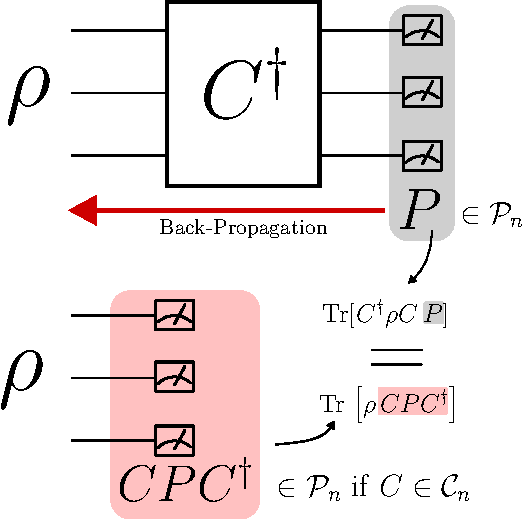
\includegraphics[width=1\linewidth]{figures/backprop_simpl.pdf}
    \caption{Measurement back-propagation: measuring observable $P$ on $C^\dagger \rho C$ yields the same outcome distribution as
     measuring $C P C^\dagger$ on $\rho$. By definition of the Clifford group, $CPC^\dagger$ is also a Pauli observable if $C\in\Clifford_n$.}
    \label{fig:backprop}
\end{figure}


%-----------------------------------------------------------
%-----------------------------------------------------------

\section{Quantum state certification with few Pauli measurements}
\label{section:certification}

In this section, we propose a protocol to check whether an i.i.d.\ prover correctly prepares an $n$-qubit target state in the \CEPS\ class, meaning a quantum state of the form
        \(
        \ket{\Psi} = C\left(\bigotimes_{i=1}^n \ket{\psi_i}\right),
        \)
        where $C$ is a known Clifford circuit and the $\ket{\psi_i}$ are arbitrary known single-qubit states, possibly including magic states.

        Without loss of generality, we can write the product state $\bigotimes_{i=1}^n\ket{\psi_i}$ by concentrating its stabilizer part in the first $s$ qubits, leaving the non-stabilizer states in the remaining $t$ qubits, with $n=s+t$ (the corresponding reordering of the qubits is a Clifford operation, which we include in $C$).
            This allows to re-write the state as $C^\dagger\ket\Psi=\ket{\psi_S}\otimes\bigotimes_{i\in M}\ket{\psi_i}$, where $S=\{1,\dots,s\}$, $M=\{s+1,\dots,n\}$, and $\ket{\psi_S}=\bigotimes_{i\in S}\ket{\psi_i}$ is a stabilizer state on $s$ qubits\footnote{If $s=0$, we keep the block $S$, with $\ket{\psi_S}$ the trivial state and $\norm{\chi_{\psi_S}}_1=1$.}. We thus see $C^\dagger\ket\Psi$ as a product state on $1+t$ blocks, labelled by $b\in\{S\}\cup M$: the block $S$, and one block for each qubit $i\in M$.

            We now define some notations. For
            $N\in\mathbb
            N$, let $\rho^{\otimes N}$ be $N$ copies of an unknown, possibly mixed, $n$-qubit quantum state.
            Let $\np=\sum_b \norm{\chi_{\psi_b}}_1=1+\sum_{i\in M}\norm{\chi_{\psi_i}}_1\le 1+t\sqrt2$. We define the probability distribution on blocks $b\in\{S\}\cup M$:
            \begin{equation}
            \label{mu_i}
                \mu(b) \coloneqq \frac{\norm{\chi_{\psi_b}}_1}m.
            \end{equation}
            For all $b\in\{S\}\cup M$, we also define the probability distributions over Pauli operators on block $b$
            \begin{equation}
            \label{Dpsi_iP}
                \mathcal{D}_{\psi_b}(P) \coloneqq \frac{|\chi_{\psi_b}(P)|}{\norm{\chi_{\psi_b}}_1}.
            \end{equation}
            Sampling $b=S$ corresponds to a test of the stabilizer block, with probability $\mu(S)=1/m$, and $\mathcal{D}_{\psi_S}$ is the uniform distribution over the stabilizer group of $\ket{\psi_S}$ (see section~\ref{subsection:prelims:DFE}). Sampling $b=i\in M$ corresponds to a test of the non-stabilizer qubit $i$, with a probability $\mu(i)=\norm{\chi_{\psi_i}}_1/m$ that depends on $\ket{\psi_i}$, and $\mathcal{D}_{\psi_i}$ is a distribution over single-qubit Pauli operators.
             Finally, we define a joint probability distribution on blocks $b$ and Pauli operators $P$ on block $b$ as
             \begin{equation}
            \label{DpsiPi}
                \pdist(b, P) \coloneqq \mu(b)\pdist_{\psi_b}(P)=\frac{|\chi_{\psi_b}(P)|}m.
            \end{equation}
            By construction, this joint distribution can be sampled from classically by sampling the block $b$ from $\mu(b)$, and then the Pauli operator $P$ from $\mathcal{D}_{\psi_b}(P)$.

            We now state our \CEPS\ certification protocol, which is also described on figure \ref{fig:protocol:certification}.
            \begin{figure*}[t]
                \centering
                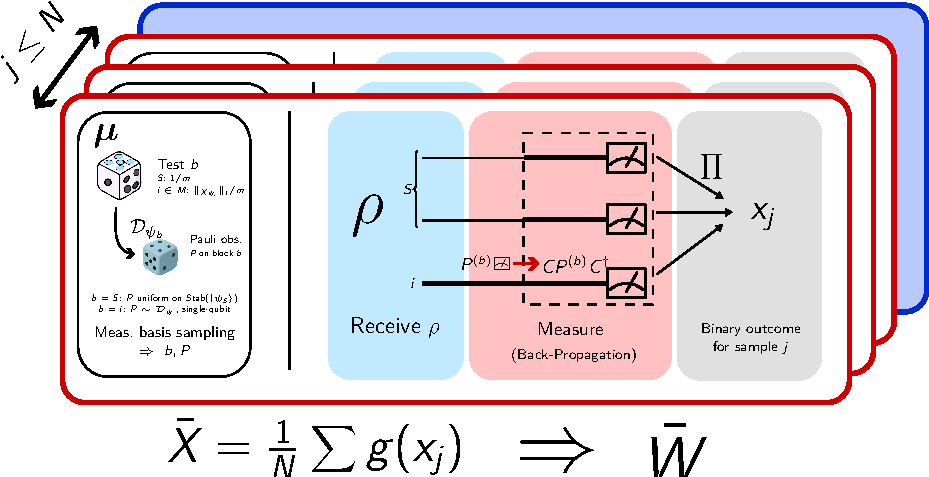
\includegraphics[width=\textwidth]{figures/sf-protocol-ceps.pdf} 
                \caption{Visual description of our protocol to certify $\mCEPS$. With the notations of Protocol \ref{protocol:certification}, here for copy $j$ for which we sampled $b, P$, we have $g(x_j) = \mathrm{sgn}(\chi_{\psi_{b_j}}(P_j)) \,x_j$. The test $b$ is either the stabilizer block $S$, with probability $1/\np$, or a non-stabilizer qubit $i\in M$, with probability $\norm{\chi_{\psi_i}}_1/\np$; here, the first two wires form the block $S$ and the last one is a qubit $i\in M$. Also, the estimate for the witness $\bar W$ is computed from the estimator $\bar X$ using $\bar W = 1-(1+t)+\np\times \bar X$.
                The samples in red boxes are used for certification, while
                the blue box is a sample that is untouched, left to be used for the computation.}
                \label{fig:protocol:certification}
            \end{figure*}

        
        %Before providing the technical details, we give a high-level description of the protocol (see Fig.~\ref{fig:protocol}). 
        %We assume that the i.i.d.\ prover prepares a state $\rho$ over $n$ qubits at each round.
        %Protocol \ref{protocol:certification} uses i.i.d.\ Pauli measurements on $N$ copies of the unknown state $\rho$ in order to estimate a robust witness of the fidelity $F(\rho,\ket\Psi)$, as in Eq.~\eqref{eq:prelims:witness}, up to precision $\epsilon$ with probability $1-\delta$. As explained in section \ref{subsection:prelims:witness}, estimating the witness requires estimating single-qubit fidelities, which can be done efficiently using DFE (section \ref{subsection:prelims:DFE}). Of course, this works only if we are able to exploit the tensor product structure of \(\ket{\Psi} = C\left(\bigotimes_{i=1}^n \ket{\psi_i}\right)\), meaning if we are able to undo the effect of $C$ on a copy $\rho$ sent by the prover. Since the verifier does not have the quantum capabilities to apply $C^\dagger$, we take advantage that only Pauli measurements are required, so the application of $C^\dagger$ can be emulated by a change of Pauli basis and classical post-processing of the outcomes, \emph{via} back-propagation (\ref{subsection:prelims:backprop}). 
        %Altogether, via an analysis using Hoeffding's inequality (section \ref{lemma:prelim:hoeffding}), we show that the sample complexity scales as $N\sim O(n^2/\epsilon^2 \; \log(1/\delta))$.

        %Informally, the protocol can be described as follows. First, the verifier associates to each qubit $i$ a weight that equals the $\ell-1$ norm of its the characteristic function of $\ket{\psi_i}$, \emph{i.e.}\ the $i-$th state of the tensor product before the Clifford. Then, for each qubit, we follow the approach of DFE in the single-qubit case. Namely, for $i\leq n$ we define a probability distribution on single-qubit Pauli operators $\pdist_i$. We call the joint probability distribution $\jdist$. For each copy, the verifier samples a qubit and a Pauli associated to this qubit from $\jdist$, back-propagated the Pauli observable and performs the measurement. The outcomes are then aggregated as if the fidelities were computed individually, but globally their estimates are being mutually summed to build an estimator of $\sum_i F(C^\dagger(\rho)_i, \ket{\psi_i})=\sum_i F(\rho_i, \ket\Psi_i)$, which is proportional to the witness by Eq. \eqref{eq:prelims:witness}. Using Hoeffding allows us to derive a lower bound on $N$ to reach the desired guarantee.


        \begin{protocol}[Certification of \CEPS]
            \label{protocol:certification}
            Let $\ket\Psi = C\left(\bigotimes_{\qubit=1}^n\ket{\psi_\qubit}\right)$ be the target state to certify and let $\epsilon>0$ be a threshold of acceptance. With the notations above, the protocol goes as follows:
            \begin{enumerate}
                \item For each copy $\copyindex\leq N$, sample classically $(b_j, P_j)\sim \pdist$, then measure $C P_j^{(b_j)} C^\dagger$ on $\rho$ (where $P^{(b)}$ denotes the $n$-qubit Pauli operator acting as $P$ on block $b$ and as identity on all the other qubits), obtaining the outcome $x_j\in\{-1, 1\}$.
                \item Compute $\bar X \coloneqq \frac{1}{N}\sum_{\copyindex=1}^N \mathrm{sgn}(\chi_{\psi_{b_j}}(P_j)) \,x_j
                $.
                \item Output $\bar W\coloneqq 1-(1+t)+\np\times \bar X$. Accept if $\bar W\ge1-\frac23\epsilon$, reject otherwise.
            \end{enumerate}
        \end{protocol}

        At a high level, Protocol~\ref{protocol:certification} uses back-propagation (see section~\ref{subsection:prelims:backprop}) to reduce the estimation of the fidelity witness on $\rho$ to its estimation on $C^\dag\rho C$. This recovers the product structure of the target state $C^\dag\ket\Psi=\ket{\psi_S}\otimes\bigotimes_{i\in M}\ket{\psi_i}$, so that the fidelities between reduced states of $C^\dag\rho C$ and the corresponding blocks of the target state can be estimated block by block via DFE (see section~\ref{subsection:prelims:DFE}). DFE is efficient here: for the stabilizer block $\ket{\psi_S}$, its cost does not depend on the number of qubits $s$, and for each non-stabilizer qubit $\ket{\psi_i}$, $d=2$. This DFE requires more samples when $\ket{\psi_i}$ is a magic state, so to compensate for this the blocks $b$ to compare are randomly selected using importance sampling via the $\mu(b)$ distribution, which gives the stabilizer block the weight of a single stabilizer qubit. The Pauli operators to measure on block $b$ are then sampled from $\mathcal{D}_{\psi_b}$, as in DFE. These fidelities are then combined to estimate the block fidelity witness of $F(C^\dag\rho C,C^\dag\Psi C)=F(\rho,\ket\Psi)$ (see section~\ref{subsection:prelims:witness}).

        Protocol~\ref{protocol:certification} only requires single-qubit Pauli measurements and simple classical post-processing (sampling from univariate distributions and from the stabilizer group of $\ket{\psi_S}$), making it time efficient in $N$ and $n$. We now show that this protocol provides a certification of the target \CEPS\ $\ket\Psi$ that is also sample-efficient:

        \begin{theorem}[Efficient certification of \CEPS]
            Let $\epsilon,\delta>0$. With the notations of Protocol~\ref{protocol:certification}, assuming $N\ge N_{iid}$ where 
            \begin{equation}
            \label{eq:certification:sample iid}
            N_{iid}\in\O\left(
                    \frac{(1+t)^2}{\epsilon^2} \log\left(\frac{1}{\delta}\right)
                    \right)
                    \; ,
            \end{equation}
                 then Protocol~\ref{protocol:certification} rejects if $F(\rho,\ket\Psi)<1-\epsilon$ and accepts if $F(\rho,\ket\Psi)\ge1-\frac\epsilon{3(1+t)}$\footnote{The constant $\frac13$ is chosen for simplicity and can be replaced by $1-\frac2k$ for any $k\in\mathcal O(1)$ with a constant increase in sample complexity, by replacing the acceptance condition in step 3 of Protocol~\ref{protocol:certification} by $\bar W\ge1-(1-\frac1k)\epsilon$ and setting $\lambda=\frac\epsilon k$ in the proof.}, with probability greater than $1-\delta$.
        \end{theorem}

        \begin{proof}
        Recall that $\jdist$ is a joint probability distribution over blocks and Pauli observables on these blocks. We define the estimator
        \begin{equation}
        \label{def_f}
            f(b,P,x)\coloneqq \sgn(\chi_{\psi_b}(P)) \times x\;,
        \end{equation}
            where $(b,P)\sim\mathcal D$ and $x\in\{+1, -1\}$ is a random variable describing the binary outcome of measuring the observable $C P^{(b)}C^\dagger$ on $\rho$ (where $P^{(b)}$ denotes the $n$-qubit Pauli operator acting as $P$ on block $b$ and as identity on all the other qubits). Then, the quantity $\bar X$ computed at step $2$ of Protocol~\ref{protocol:certification} using $N$ samples $(b_j,P_j,x_j)$ is an empirical estimate of the expected value of $f$ over the classical randomness of $(b,P)$ and the quantum randomness of $x$, which writes $X=\mathbb E_{b,P,x}[f(b,P,x)]$.
        
        Now we have:
        \begin{align}
            X &= \mathbb E_{b,P,x}[f(b,P,x)]\\
            &=
            \sum_{b}
            \mu(b)
            \sum_{P\in\Pauli_{|b|}}
            \pdist_{\psi_b}(P)
            \,\sgn(\chi_{\psi_b}(P))\\
            \nonumber&\quad\quad\quad\quad\quad\quad\quad\quad\times\Tr[\rho \; C P^{(b)} C^\dagger]
            \\
            &=
            \sum_{b}
            \sum_{P\in\Pauli_{|b|}}
            \dfrac{\norm{\chi_{\psi_b}}_1}{\np}
            \,\dfrac{|\chi_{\psi_b}(P)|}{\norm{\chi_{\psi_b}}_1}\\
            \nonumber&\quad\quad\quad\quad\times\sgn(\chi_{\psi_b}(P))\Tr[\rho \; C P^{(b)} C^\dagger]
            \\
            &=
            \sum_{b}
            \sum_{P\in\Pauli_{|b|}}
            \dfrac{|\chi_{\psi_b}(P)|}{\np}
            \,\sgn(\chi_{\psi_b}(P))\\
            \nonumber&\quad\quad\quad\quad\quad\quad\quad\quad\times\Tr[\rho \; C P^{(b)} C^\dagger]
            \\
            &=
            \dfrac{1}{\np}
            \sum_{b}
            \sum_{P\in\Pauli_{|b|}}
            \chi_{\psi_b}(P) \Tr[\rho \; C P^{(b)} C^\dagger]
            \\
            &=
            \dfrac{1}{\np}
            \sum_{b}
            \sum_{P\in\Pauli_{|b|}}
            \chi_{\psi_b}(P) \Tr[C^\dagger\rho C \; P^{(b)} ]
            \\
            &=
            \dfrac{1}{\np}
            \sum_{b}
            \sum_{P\in\Pauli_{|b|}}
            \chi_{\psi_b}(P) \Tr[(C^\dagger\rho C)_b \; P ]
            \\
            &=
            \dfrac{1}{\np}
            \sum_{b}
             \Tr[(C^\dagger\rho C)_b \; \ketbra{\psi_b} ]
            \\
            &=
            \dfrac{1}{\np}
            \sum_{b}
             F((C^\dagger\rho C)_b, (C^\dagger\Psi C)_b),
        \end{align}
        where we used Eq.~\eqref{def_f} and the Born rule in the second line, Eqs.~\eqref{mu_i} and~\eqref{Dpsi_iP} in the third line (where the sums run over the $1+t$ blocks $b\in\{S\}\cup M$ and over the Pauli operators $P$ on the $|b|$ qubits of block $b$), the simplification $\mu(b)\,\pdist_{\psi_b}(P)=|\chi_{\psi_b}(P)|/\np$ of Eq.~\eqref{DpsiPi} in the fourth line, $|\chi_{\psi_b}(P)|\,\sgn(\chi_{\psi_b}(P))=\chi_{\psi_b}(P)$ in the fifth line, the cyclicity of the trace in the sixth line, where in the seventh line $(C^\dag\rho C)_b$ denotes the reduced state of $C^\dag\rho C$ on block $b$, and where we used Eq.~\eqref{expansion} in the eighth line and Eq.~\eqref{fidover} in the last line.
        
        With Eq.~\eqref{eq:prelims:blockwitness} applied to these $1+t$ blocks, we thus obtain 
        \begin{equation}
            \label{eq:equality witness sum of fid}
            W(C^\dagger\rho C,C^\dagger\Psi C) = 1-(1+t)+\np X\; .
        \end{equation}

        Next, we show how close the empirical estimate $\bar X=\frac1N\sum_{j=1}^Nf(b_j,P_j,x_j)$ is to $X=\mathbb E_{b,P,x}[f(b,P,x)]$. Since the range of $f$ is $\max_{b,P,x}f(b,P,x)-\min_{b,P,x}f(b,P,x)\leq2$, Hoeffding's inequality (see Lemma \ref{lemma:prelim:hoeffding}) implies
        \begin{equation}
            \Pr[
            |\bar X - X| \geq \lambda
            ] \leq \exp
            \left(
            -\frac12N\lambda^2
            \right),
        \end{equation}
        for any $\lambda>0$.
        Furthermore, by Eq.\ (\ref{eq:equality witness sum of fid}) we have $W=1-(1+t) +\np X$, so
        \begin{equation}
            \begin{aligned}
            \mathrm{Pr}[
            |\bar W - W| \geq \lambda
            ] &= 
            \mathrm{Pr}\left[
            |\bar X - X| \geq \dfrac{\lambda}{\np}
            \right] \\
            &\leq
            \exp{
            \left(
            -\dfrac{N \lambda^2}{2\np^2}
            \right)
            },
            \end{aligned}
        \end{equation}
        which is smaller than $\delta>0$ as soon as $N\ge N(\lambda)$ where
            \begin{equation}
                N(\lambda)\coloneqq\frac{2\np^2}{\lambda^2}\log\left(\dfrac{1}{\delta}\right)\; .
            \end{equation}
 
        By cyclicity of the trace we have $F(C^\dagger\rho C,C^\dagger\Psi C)=F(\rho,\ket\Psi)$ so Eq.~\eqref{eq:prelims:blockwitness:robustness} with $B=1+t$ implies
        \begin{equation}
            \begin{aligned}
            1-(1+t)(1-F(\rho,\ket\Psi)) &\leq W(C^\dagger\rho C,C^\dagger\Psi C)\\
            &\leq F(\rho,\ket\Psi).
            \end{aligned}
        \end{equation}
        Hence, with probability greater than $1-\delta$, $N\ge N(\lambda)$ implies
        \begin{equation}
            1-(1+t)(1-F(\rho, \ket\Psi)) -\lambda \leq \bar W \leq F(\rho, \ket\Psi) + \lambda\; .
        \end{equation}
        In particular, the right hand side shows that $F(\rho,\ket\Psi)<1-\epsilon$ implies $\bar W<1-\epsilon+\lambda$, while the left hand side shows that $F(\rho,\ket\Psi)\ge1-\frac\epsilon{3(1+t)}$ implies $\bar W\ge1-\epsilon/3-\lambda$. Setting $\lambda=\epsilon/3$ concludes the proof, with $N_{iid}=N(\epsilon/3)\in\mathcal O(\frac{(1+t)^2}{\epsilon^2}\log(\frac{1}{\delta}))$ since $m\le 1+t\sqrt2$.
        \end{proof}
        As a result, we can efficiently certify any $n-$qubit state of the $\mCEPS$ class using only (non-adaptive) single-qubit Pauli measurements on a number of samples that scales quadratically in the number $t$ of non-stabilizer states $\ket{\psi_i}$, independently of the number $s$ of stabilizer ones, and with efficient sampling and post-processing of measurement outcomes.
 

%-----------------------------------------------------------

\section{State verification in the adversarial scenario}
\label{section:verification}

In many quantum verification tasks, security or correctness analyses rely on the assumption that all copies of the quantum state are produced independently and identically distributed (i.i.d.).
In an adversarial scenario, however, this assumption may fail: the subsystems across different rounds can be arbitrarily correlated.
The following result, adapted directly from~\cite[Theorem~3]{FKMO24learning}, shows that for protocols requiring non-adaptive, single-copy (incoherent) measurements only, the same estimation guarantees obtained in the i.i.d.\ case can still be achieved in the general, non-i.i.d.\ case — at the price of requiring a larger number of total samples, which is captured by Lemma \ref{lemma:prelim:iid}.

\begin{lemma}[State certification in the non-i.i.d.\ setting {\cite[Theorem~3]{FKMO24learning}}]
\label{lemma:prelim:iid}
Let $\mathcal A$ be a protocol that, given $N_{{iid}}\in\mathbb N$ i.i.d.\ copies of an $n$-qubit state $\rho$ (single-copy dimension $d=2^n$), performs non-adaptive, single-copy (incoherent) measurements and outputs a flag $\Accept/\Reject$ such that
\begin{equation}
    \Pr\left[\mathcal A(\rho^{\otimes N_{iid}}) = \Accept \; |\;  F(\rho, \ket\Psi) < 1-\epsilon\right] \leq \delta
\end{equation}
and
\begin{equation}
    \begin{aligned}
    \Pr\Big[&\mathcal A(\rho^{\otimes N_{iid}}) = \Reject \; |\\
    &F(\rho, \ket\Psi) \geq 1-\frac{1}{3(1+t)} \epsilon\Big] \leq \delta
    \end{aligned}
\end{equation}

Let $N_{{non-iid}}>N_{{iid}}$. Consider the protocol $\mathcal B$ that, on an arbitrary joint state $\rho^{1\ldots N_{{non-iid}}}\in(\Hilbert^{\otimes n} )^{\otimes N_{non-iid}}$, randomly permutes the subsystems, discards $N_{non-iid}-N_{{iid}}-1$ of them uniformly at random, applies $\mathcal A$ to the remaining $N_{\mathrm{iid}}$ subsystems, and leaves one held-out final subsystem.
Then, for the (uniformly random) held-out subsystem $\rho^{\mathrm{fin}}$,
\begin{equation}
    \Pr\left[\mathcal B(\rho) = \Accept \; |\;  F(\rho^{\mathrm{fin}}, \ket\Psi) < 1-\epsilon\right] \leq \delta
\end{equation}
and
\begin{equation}
    \begin{aligned}
    \Pr\Big[&\mathcal B(\rho) = \Reject \; |\\
    &F(\rho^{\mathrm{fin}}, \ket\Psi) \geq 1-\frac{1}{3(1+t)} \epsilon\Big] \leq \delta
    \end{aligned}
\end{equation}
whenever
\[
N_{{non-iid}}\in\Omega\!\left(
\frac{\log d}{\delta^2\epsilon^2}\,N_{{iid}}^{\,2}\,
\log^2\!\Big(\frac{N_{{iid}}}{\delta}\Big)
\right).
\]
\end{lemma}

\begin{figure}
    \centering
    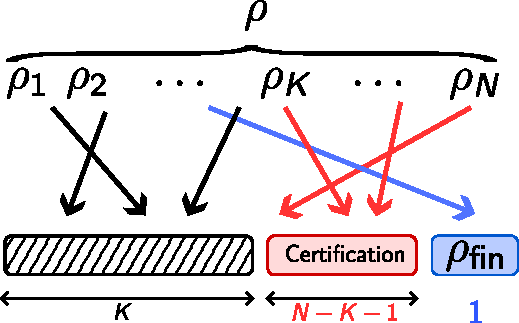
\includegraphics[width=\linewidth]{figures/adversarial.pdf}
    \caption{Illustration of the protocol to run against an adversarial prover. The verifier receives different $n-$qubit subsystems of a global system $\rho^{1\ldots N}\in(\Hilbert^{\otimes n} )^{\otimes N}$
    The verifier chooses a random partition, discards $K$ systems, applies the certification protocol}
    \label{fig:adversarial}
\end{figure}
An intuitive depiction of the protocol described by lemma \ref{lemma:prelim:iid} can be found in figure \ref{fig:adversarial}.


We have proven the security of Protocol \ref{protocol:certification} under the assumption that the incoming state is of the form $\rho^{\otimes N}$, meaning that the states are produced in an independent and identically distributed way. In an adversarial scenario, this is not necessarily the case. In Protocol \ref{protocol:verification}, we thus increase the number of samples and randomly partition the subsystems before applying Protocol \ref{protocol:certification} on a subset of registers in order to use the results of lemma \ref{lemma:prelim:iid}.

\begin{protocol}[Verification of \CEPS]
\label{protocol:verification}

Let $\ket\Psi = C\left(\bigotimes_{\qubit=1}^n\ket{\psi_\qubit}\right)$ be the target state to certify, $\epsilon>0$ be a threshold of acceptance. Also, let $N_1,N_2\in\mathbb N$ be such that $N_1>N_2$. Denoting by $\rho^{1\ldots N_1}\in(\Hilbert^{\otimes n})^{\otimes N_1}$ the state prepared by the prover,
% sent in $N_1$ registers of $n$ qubits,
the protocol goes as follows. The verifier first chooses a random partition of the set $\{1, \ldots, N_1\}$ of $3$ subsets with respective size and labels: 
size $N_{2}$ (\texttt{test}), $N_1-N_2-1$ (\texttt{discard}), and $1$ (\texttt{keep}). Then, for each received register $j\leq N_1$:
\begin{itemize}
    \item Discard the received registers $j\in \texttt{discard}$.
    \item Run Protocol \ref{protocol:certification} on registers $j\in \texttt{test}$. Output an acceptance/rejection flag.
    \item Keep register $j\in\texttt{keep}$, with the above flag.
\end{itemize}
\end{protocol}
     \begin{theorem}[Efficient verification of \CEPS]
            Let $\epsilon,\delta>0$. With the notations of Protocol~\ref{protocol:verification}, assuming 
            % $N_1\ge N_{non-iid}$ where $N_{non-iid}\in\tilde \Omega\left(\frac{n^5}{\delta^2 \epsilon^6}\right)$,
            $N_2\ge N_{iid}\in\O(\frac{(1+t)^2}{\epsilon^2}\log(1/\delta))$,
            and
            \(
            N_1\in\Omega\!\left(
            \frac{n}{\delta^2\epsilon^2}\,N_{{iid}}^{\,2}\,
            \log^2\!\Big(\frac{N_{{iid}}}{\delta}\Big)
            \right),
            \)
            then Protocol~\ref{protocol:verification} rejects if $F(\rho^{\mathrm{fin}},\ket\Psi)<1-\epsilon$ and accepts if $F(\rho^{\mathrm{fin}},\ket\Psi)\ge1-\frac\epsilon{3(1+t)}$\footnote{See previous note for the constant $\frac13$.}, with probability greater than $1-\delta$.
        \end{theorem}


        As a corollary of the above, verifying a $n-$qubit state of the \CEPS~ class with precision $\epsilon$ and failure probability at most $\delta$ requires a total number of samples $N_1\geq N_{non-iid}$ where
        \begin{equation}
            \label{eq:verification:scaling}
        N_{non-iid} \in \tilde\O\left(\frac{n(1+t)^4}{\delta^2\epsilon^6}\right)\; .
        \end{equation}
        with $\tilde O$ hiding polylogarithmic factors in $n,\epsilon, \delta$.
        The factor $(1+t)^4$ comes from the square of $N_{iid}$ in Lemma~\ref{lemma:prelim:iid}. The remaining linear factor $n$ comes from the factor $\log d=n$ in the same lemma, that is, from the dimension of the $n$-qubit registers sent by the prover, which does not depend on the structure of the target state.


        \begin{proof}
            The above theorem and corollary are easily proved using lemma \ref{lemma:prelim:iid}, as it is a particular instance of state certification in the non-i.i.d setting (what we called "state \emph{verification}") using non-adaptive and incoherent measurements according to the definitions of \cite{FKMO24learning}. Indeed, the subroutine Protocol \ref{protocol:certification} involves Pauli observables that can be sampled in advance (according to the mentioned probability distribution), therefore non-adaptive. The observables are measured on the individual subsystems separately, therefore the measurements are incoherent. Lemma \ref{lemma:prelim:iid} thus applies and sets the scaling of $N_{non-iid}$ for the verification procedure 
            in function of $N_{iid}$ of the certification procedure in order to reach the same success probability $1-\delta$ for the same target precision $\epsilon$. By simply plugging the scaling of $N_{iid}$ in the formula of $N_{non-iid}$, we get \eqref{eq:verification:scaling}.
        \end{proof}
\section{Verification of universal quantum computations}
\label{section:VQC}
    % Whether we are in the \emph{i.i.d} or \emph{non-i.i.d} setting, we have shown that we can provide a witness of the fidelity of the last remaining subsystem to the target state, or more an estimate of the witness up to precision $\epsilon$ with success probability $\geq 1-\delta$. In particular, the witness lower bounds the fidelity. In the context of quantum computing \emph{via} magic-state injection, we have seen that any quantum computation can be compiled in a way that a Clifford-enhanced Product State can be associated to it, with as many magic-states in it as there are non-Clifford operations, and that only (adaptive) Pauli measurements remain to be performed on the remaining state to yield the outcome of the intended computation. Hence, since a witness of the fidelity of the remaining state to the target state is provided, we conclude using the Fuchs--van de Graaf inequalities (Eq.~\eqref{eq:prelim:fuchsvandegraaf}) that the trace distance between the actual and the ideal output state is at most $\sqrt{\epsilon}$, implying that their measurement statistics---and hence the computational outcome distributions---differ by at most $\sqrt{\epsilon}$.
   

As stated in the introduction, the computation model that we consider is the Magic-State Injection model of \cite{BK04universal}, in which the computation is performed by preparing a state $\ket\Psi\in\mCEPS$ and performing (adaptive) Pauli measurements on it. Let $P_{adapt}$ be the procedure that outputs a Pauli basis for the $i-th$ qubit based on the measurement outcomes of the $1...i-1$ qubits, conformly to the MSI model.


In this section, we show that verifying the outcome of such a computation can be reduced to certifying the state $\ket\Psi$, by using as main argument the Fuchs-Van-De-Graaf inequalities as teased in the preliminaries.  
\begin{protocol}
    \label{protocol:verification of UQC}
    Let $\ket\Psi$ be the $\mCEPS$ state associated to the target computation,
    and $P_{adapt}$ be the adaptive Pauli measurements to perform on $\ket{\Psi}$.
    The protocol then goes as follows, when the Prover sends $\rho\in\Hilbert^{\otimes N}$
    \begin{enumerate}
        \item Run Protocol \ref{protocol:certification} (i.i.d prover)/Protocol \ref{protocol:verification} (non-i.i.d prover) on $\rho$, output an acceptance/rejection flag, and a remaining subsystem whose reduced state is $\rho^{\mathrm{fin}}$. If the flag is $\Accept$, move to the next step, else abort.
        \item Perform the adaptive Pauli measurements on $\rho^{\mathrm{fin}}$, let the result be $\rho_{\mathrm{res}}= P_{adapt}(\rho^{\mathrm{fin}})$.
    \end{enumerate}
\end{protocol}

The above protocol therefore uses the state certification/verification procedures to output a flag, indicator of the closeness of the remaining untouched register to the target state. Note that this procedure uses non-adaptive Pauli measurements only, which allowed us to lift the i.i.d assumption as mentioned in previous section.
Once this is done, the adaptive Pauli measurements required for the target computation can be performed on the remaining register. As next theorem shows, the guarantee on the closeness of the prepared state to the target state can be lifted to a guarantee on the closeness of the distributions of the computation outcomes,  per the Fuchs-Van-De-Graaf inequalities.

As a corollary, verification of universal quantum computations is thus achieved with $N\geq N_{iid}$ or $N\geq N_{non-iid}$ depending on the assumptions made on the prover, and with the scalings computed above, in \eqref{eq:certification:sample iid} and \eqref{eq:verification:scaling} respectively.

\begin{theorem}[Efficient verification of MSI-based quantum computation]
    Let $\epsilon, \delta >0$. With the notations of Protocol \ref{protocol:verification of UQC}, 
    let $\ket{\Psi_{out}} = P_{adapt}(\ket\Psi)$ be the ideal outcome of the computation. In the case of acceptance, let $\rho_{\mathrm{res}} = P_{adapt}(\rho^{\mathrm{fin}})$ be the actual output of the computation. Then,
    the outcomes distributions differ (in trace distance) by at most
        $D(\rho_{\mathrm{res}}, \ket{\Psi_{out}}) \leq \sqrt\epsilon$, with probability $\geq 1-\delta$
        .
\end{theorem}


\begin{proof}
    In the acceptance situation, with probability $\geq 1-\delta$ we have $F(\rho^{\mathrm{fin}}, \ket\Psi) \geq 1-\epsilon$. By the Fuchs-Van-De-Graaf inequalities, this implies that $D(\rho^{\mathrm{fin}}, \ket\Psi) \leq \sqrt{1-F(\rho^{\mathrm{fin}}, \ket\Psi)} \leq \sqrt{\epsilon}$, with probability $\geq 1-\delta$. Since $P_{adapt}$ is a measurement procedure performed on these states, this trace distance also holds for the measurement outcomes, hence the conclusion of the proof.
\end{proof}
%-----------------------------------------------------------


% \section{Quantum state verification with few Pauli measurements}

% \begin{itemize}
%     \item Iid robust hypothesis testing
%     \item Beyond iid hypothesis testing
%     \item How we do it
%     \item Corollary: Verification of universal quantum computations: non-adaptive vs adaptive measurements
% \end{itemize}


%-----------------------------------------------------------


\section{Conclusion}
\label{section:conclusion}

In this work, we have introduced an efficient and experimentally feasible protocol for certifying Clifford-enhanced Product States (\CEPS), a natural class of resource states for Magic-State Injection (MSI), prominent model in
% fault-tolerant
quantum computing architectures.

In the \emph{i.i.d} case, our \emph{state certification} is conducted by an estimate of a robust fidelity witness for the received state to the target state, a quantity that notably lower bounds the fidelity \cite{CGKM21efficient}. This yielded in an efficient protocol to certify $\mCEPS$ using Pauli measurements only: the first for this class of states.

In the \emph{non-i.i.d} case, \emph{state verification} can be conducted in the same way, at the cost of a larger sample
complexity (still polynomial in $n$) and with a verifier "subsystem shuffling" phase. This uses the result of \cite{FKMO24learning}, but we suspect that a better sample complexity can be obtained by analyzing this problem through the lenses of sampling without replacement in the hypothesis testing framework as it has been done in \cite{LZH23robust}. 

Crucially, verifying an MSI-based quantum computation naturally follows from our certification/verification protocols, requiring only simple Pauli measurements and classical post-processing. Our protocols thus remain compatible with current and near-term fault-tolerant architectures, imposing minimal additional overhead on the verifier.




 This work thus presents the first efficient solution for the problem of verification of quantum computations expressed in the MSI model relying on single-qubit Pauli measurements only. It indeed stands in contrast to the existing approaches for other models like MBQC (involving Graph states and Hypergraph states verification) or general Pauli-based state certification techniques that requires a description of the quantum state that is $\#P-$hard to obtain in the present case \cite{YJS18quantum}. 
 We expect that this simplicity and scalability will make verification of MSI-based computations an appealing direction for both theoretical study and experimental implementation in near-term quantum platforms.

In particular, it would be interesting to investigate whether the sample complexity in the adversarial setting can be improved using sampling-without-replacement techniques, and whether the class of certifiable states can be broadened by considering back-propagation of observables in other computation models like the coherence-based, rather than the magic-based (Clifford/non-Clifford) framework adopted here.

 

 







\section*{Acknowledgements}

UC thanks D.\ Leichtle for inspiring discussions.
SAS acknowledges H.\ Thomas and V.\ Upreti for feedbacks on figures and fruitful discussions. MG acknowledges funding from the Hybrid Quantum Initiative (HQI) supported by France 2030 under ANR
grant ANR-22-PNCQ-0002.


% \printbibliography
\bibliographystyle{linksen}
\bibliography{bibliography}

\appendix

\section{$\ell_1-$norm of CPS states}
A $n-$qubit state
$\ket{\Psi} \in \mCEPS$ is of the form $C\left(\bigotimes_{i=1}^n\ket{\psi_i}\right)$. Let us analyze the $\ell_1-$norm of $\chi_{\Psi}$, the characteristic function of such a state, defined by
\begin{equation}
    \norm{\chi_\Psi}_{\ell_1} = \dfrac{1}{2^n}\sum_{P\in\Pauli_n\backslash\{\mathds{1}_n\}} \abs{\Tr[P\rho]}
\end{equation}
where $\rho = \ketbra\Psi$. By cyclicity of the trace, and denoting $P = P_1\otimes P_2\otimes ... \otimes P_n$, we have
\begin{widetext}
\begin{align}
    \norm{\chi_\Psi}_{\ell_1} 
    &= \dfrac{1}{2^n}\sum_{P\in\Pauli_n\backslash\{\mathds{1}_n\}} \abs{
        \Tr[P\rho]
        }
        \\
    &= \dfrac{1}{2^n}\sum_{P\in\Pauli_n\backslash\{\mathds{1}_n\}} \abs{
        \Tr\left[ 
            \left( 
                C{(P_1 \otimes P_2 \otimes \cdots \otimes P_n)}C^\dagger  
                \right)
                \left( \bigotimes_{i=1}^n \ketbra{\psi_i} \right)
                \right]
        }
        \\
    &= \dfrac{1}{2^n}\sum_{P\in\Pauli_n\backslash\{\mathds{1}_n\}} \abs{
        \Tr\left[ 
            \left( 
                \tilde P_1 \otimes \tilde P_2 \otimes \cdots \otimes \tilde P_n
                \right)
                \left( \bigotimes_{i=1}^n \ketbra{\psi_i} \right)
                \right]
        }
        \\
    &= \dfrac{1}{2^n}\sum_{P\in\Pauli_n\backslash\{\mathds{1}_n\}} \abs{
        \prod_{i=1}^n
        \Tr\left[ 
                \tilde P_i \; \rho_i
                \right]
        }
\end{align}
\end{widetext}

where we used $\tilde P = CPC^\dagger\in\Pauli_n$, and $\rho_i = \ketbra{\psi_i}$. We now analyze the worst-case scenario where $\rho_i = \rho_T = T\ketbra{+}T^\dagger$. For these states, $\Tr[X\rho_T]=\Tr[Y\rho_T]=1/\sqrt 2$ while $\Tr[Z\rho_T]=0$, and obviously $\Tr[\mathds 1\rho_T] = 1$. In this situation, computing the above expression becomes simply a counting problem.
\begin{itemize}
    \item Counting the number of $n-$qubit Paulis that have at least one $Z$: they contribute by $0$ to the sum
    \item Counting the number of $n-$qubit Paulis that have $i$ indices equal to $\mathds 1$ and $n-1$ indices equal to $X$ or $Y$: they contribute by $1^i \times (1/\sqrt2)^{n-i}$ to the sum ; for $0\leq i \leq n-1$.
\end{itemize}

We see that the only relevant terms are the ones with $i$ $\mathds 1$ and $n-i$ $X/Y$. So we hereby define
\begin{equation}
    \Pauli_n^{(i)} = \left\{
        P\in\Pauli_n
        \quad | \quad
        W_{\mathds{1}}(P)\geq i
        \; \wedge \;
        W_{Z}(P)=0
    \right\}
\end{equation}
where $W_{\mathds 1}(P)$ denotes the weight of the $n-$qubit Pauli $P$ with respect to single-qubit Pauli $\mathds 1$, meaning the number of indices in $P$ that equal $\mathds{1}$. Thus, we reduced the $\ell_1-$norm of the worst-case $n-$qubit CPS case to 
\begin{align}
    \norm{\chi_\Psi}_{\ell_1} 
    &= 
    \dfrac{1}{2^n}
    \sum_{\Pauli_n^{(i)}}
    (1/\sqrt2)^{n-i}
    \\
    &= 
    \dfrac{1}{2^n}
    \sum_{i=0}^{n-1}
    \sum_{P\in\Pauli_n^{(i)}}
    (1/\sqrt 2)^{n-i}
    \\
    &= 
    \dfrac{1}{2^n}
    \sum_{i=0}^{n-1}
    (1/\sqrt 2)^{n-i}
    \times 2^{n-i}
    \begin{pmatrix}
        n\\
        i
    \end{pmatrix}
    \\
%     &= 
%     \dfrac 1 2
%     \sum_{i=0}^{n-1}
%     (1/\sqrt 2)^{n-i}
%     \times 2^{n-i}
%     \dfrac{n!}{i!(n-i)!}
% \end{align}
% \begin{align}
    % \norm{\chi_\Psi}_{\ell_1} 
    % &= 
    % \dfrac 1 2
    % \sum_{i=0}^{n-1}
    % \left(\frac{1}{\sqrt 2}\right)^{n-i}
    % \times 2^{n-i}
    % \dfrac{n!}{i!(n-i)!} \\[4pt]
    % &= 
    % \dfrac 1 2
    % \sum_{i=0}^{n-1}
    % \binom{n}{i}
    % \left(\frac{2}{\sqrt 2}\right)^{n-i} \\[4pt]
    \\
    &=
    \dfrac{1}{2^n}
    \sum_{i=0}^{n-1}
    \binom{n}{i}
    (\sqrt{2})^{\,n-i}.
\end{align}

We now perform a change of variable by setting $j = n-i$. As $i$ runs from $0$ to $n-1$, $j$ runs from $n$ down to $1$, so
\begin{align}
    \norm{\chi_\Psi}_{\ell_1}
    &=
    \dfrac{1}{2^n}
    \sum_{j=1}^{n}
    \binom{n}{n-j}
    (\sqrt{2})^{\,j} \\[4pt]
    &=
    \dfrac{1}{2^n}
    \sum_{j=1}^{n}
    \binom{n}{j}
    (\sqrt{2})^{\,j},
\end{align}
where we used the symmetry $\binom{n}{n-j} = \binom{n}{j}$.

Using the binomial theorem,
\begin{equation}
    \sum_{j=0}^{n} \binom{n}{j} (\sqrt{2})^j = (1+\sqrt{2})^n,
\end{equation}
so that
\begin{align}
    \sum_{j=1}^{n} \binom{n}{j} (\sqrt{2})^j
    &= (1+\sqrt{2})^n - 1.
\end{align}
Hence, for this worst-case CPS state,
\begin{equation}
    \norm{\chi_\Psi}_{\ell_1}
    = \dfrac{1}{2^n} \bigl[ (1+\sqrt{2})^n - 1 \bigr]
\end{equation}
which scales exponentially in $n$ since $1+\sqrt 2 > 2$.
\end{document}
